\chapter{An integrative network approach for MIBC subtyping} \label{s:N_I}
\chaptermark{Integrative network pipeline}


\vspace{3mm}
\fbox{
    \parbox{0.95\linewidth}{
      \begin{itemize}
        \item Developed a network pipeline and tools to analyse the outputs
        \item Mutations were integrated through edge weights 
        \item Transcription Factors integrated through selective edge pruning
        \item Use of freshly isolated samples (P0) to build a network which is then used to inform MIBC stratification
      \end{itemize}
    }
}
\vspace{3mm}


\section{Introduction}

In the previous chapter, standard clustering methods and insights from in situ experiments \citep{Baker2022-bj} were utilised to stratify the \acrfull{mibc} cohort from \acrfull{tcga}. The work revealed new MIBC subgroups with significant biological differences compared to those identified in the TCGA and consensus classifications \citep{Robertson2017-mg,Kamoun2020-tj}. This finding highlights the potential for discovering biologically relevant groups and underscores the need for new integrative methods that combine data at the computational level.

Network/Graph methods have been previously used to stratify other cancers (glioblastoma - \citet{Care2019-ij}), and the co-expressed network constitutes a method that enables further data integration, such as mutations or \acrfull{tf}. This allows for prioritising different gene sets rather than treating all of them equally, as in the case of traditional clustering models (e.g., K-means). Building a relational representation between the genes also aligns the analysis more closely with biological processes. Networks also serve as powerful visualisation tools, enhancing understanding complex processes or issues, such as the molecular depiction of cancerous tissue from gene expression.

This chapter aims to investigate how mutations and transcription factors can be integrated into a network and how healthy gene expression can inform MIBC subtyping. Apart from building the graph, there is a need to develop the tools and methods to analyse the extensive outputs, highlighting the challenges inherent in working with unsupervised learning, particularly in the context of highly heterogeneous data.

There are two networks constructed: one from the tumour dataset (Section \ref{s:N_I:tum}) and another from the healthy\footnote{Healthy he refers to the non-tumour samples from the JBU. The two terms and non-cancerous are used interchangeably throughout the thesis.} dataset (Section \ref{s:p0}). The goal of the first network type is to demonstrate the potential of the network approach and to draw comparisons with the findings from the previous chapter. The experiments with the healthy networks investigate how non-tumour gene expression can inform MIBC stratification, thus performing an integration at the graph level.

The chapter begins by presenting the methods in \cref{s:N_I:methods}, covering the network pipeline and the data integration. \Cref{s:N_I:tum} presents the work on analysing tumour networks, which compares with the cluster analysis done in previous chapter. Next, the networks built from freshly isolated samples are built and used to derived the MIBC in \cref{s:p0} as a first attempt to use gene expression from healthy cells.

% Overall, the work presented demonstrates the potential of networks in MIBC subtyping. This is enforced by the analysis and biological findings in the next \cref{s:N_I:sel_tfs} which found a subset of TF that have a high impact on both tumour and non-tumour tissues. However, the initial methods for data integration show limited impact on disease subtyping, this chapter lays the groundwork for future chapters, where initial assumptions are revised, and new, adapted methods are employed.



% Datasets
\subsection*{Datasets}

The MIBC cohort from The Cancer Genome Atlas \citep{Tcga2018-sj} and the freshly isolated cells (P0) from the Jack Birch Unit (JBU) are used in this chapter for building two different types of networks. The tumour dataset is used in the first part of the chapter to test if the integration of the mutations (from TCGA as well) amplifies the signal in the tumours and leads to different MIBC subgroups; see \cref{s:N_I:tum}. The gene expressions from P0 samples are used to build the co-expressed networks into which the mutations are integrated (using the TCGA data) from which the other MIBC subgroups are derived.

Mutation information is obtained from Whole Exome Sequencing (WES) of the MIBC cohort from TCGA, focusing specifically on the mutation count, i.e., the frequency of gene mutations across the tumour biopsies. The list of Transcription Factors is taken from The Human Transcription Factors study by \citet{Lambert2018-el}. The different aspects of the datasets are introduced in the background \cref{s:lit:datasets_used}.


% \textbf{Taken From P0 - Don't think I needed it}
% The Jack Birch's Unit holds a large dataset of bladder tissue samples both cancerous and non-cancerous. There are three different types of ' '  (i.e. non-cancerous) bladder samples: P0 (23), ABS/Ca-differentiated (49) and undifferentiated (15). The P0 are in situ tissues taken from individual with urinary tract infections (UTIs) unaltered in the lab, the ABS/Ca differentiated are in vitro which have been differentiated by the ABS/Ca protocol and lastly the undifferentiated are in vitro samples which tissues are yet not specialised; covered in \cref{s:lit:datasets_used}.From the previous classifications \citet{Robertson2017-mg, Kamoun2020-tj} it is known that there are 2 major subgroups Luminal (Lum) and Basal (Ba). The former is known to share aspects with the differentiated tissue while the latter with the undifferentiated. 


% Aims
\section{Aims}

The aim of this chapter is to validate the data integration hypothesis using both tumour and non-tumour networks:

\begin{itemize}
    \item The edge weights of a node can be modelled proportional to its mutational burden
    \item The number of connection (or degree) can be used to prioritised a subset of genes over the others
    \item A non-tumour graph representation can inform the MIBC stratification 
\end{itemize}

% This needs to be in the literature review side of things

\import{Sections/Network_I/}{methods.tex}

\newpage
\newgeometry{left=1.5cm, right=1.5cm, top=0.5cm, bottom=1cm}
\begin{figure}[p]
  \thispagestyle{empty} % Suppress the page number on this page
  \centering
  \captionsetup{justification=centering, labelfont=bf}
    \parbox{\textwidth}{\centering \Huge Tumour derived Network - Leiden} % 
  \vspace{3cm} 
    \label{fig:N_I:tum_net}
  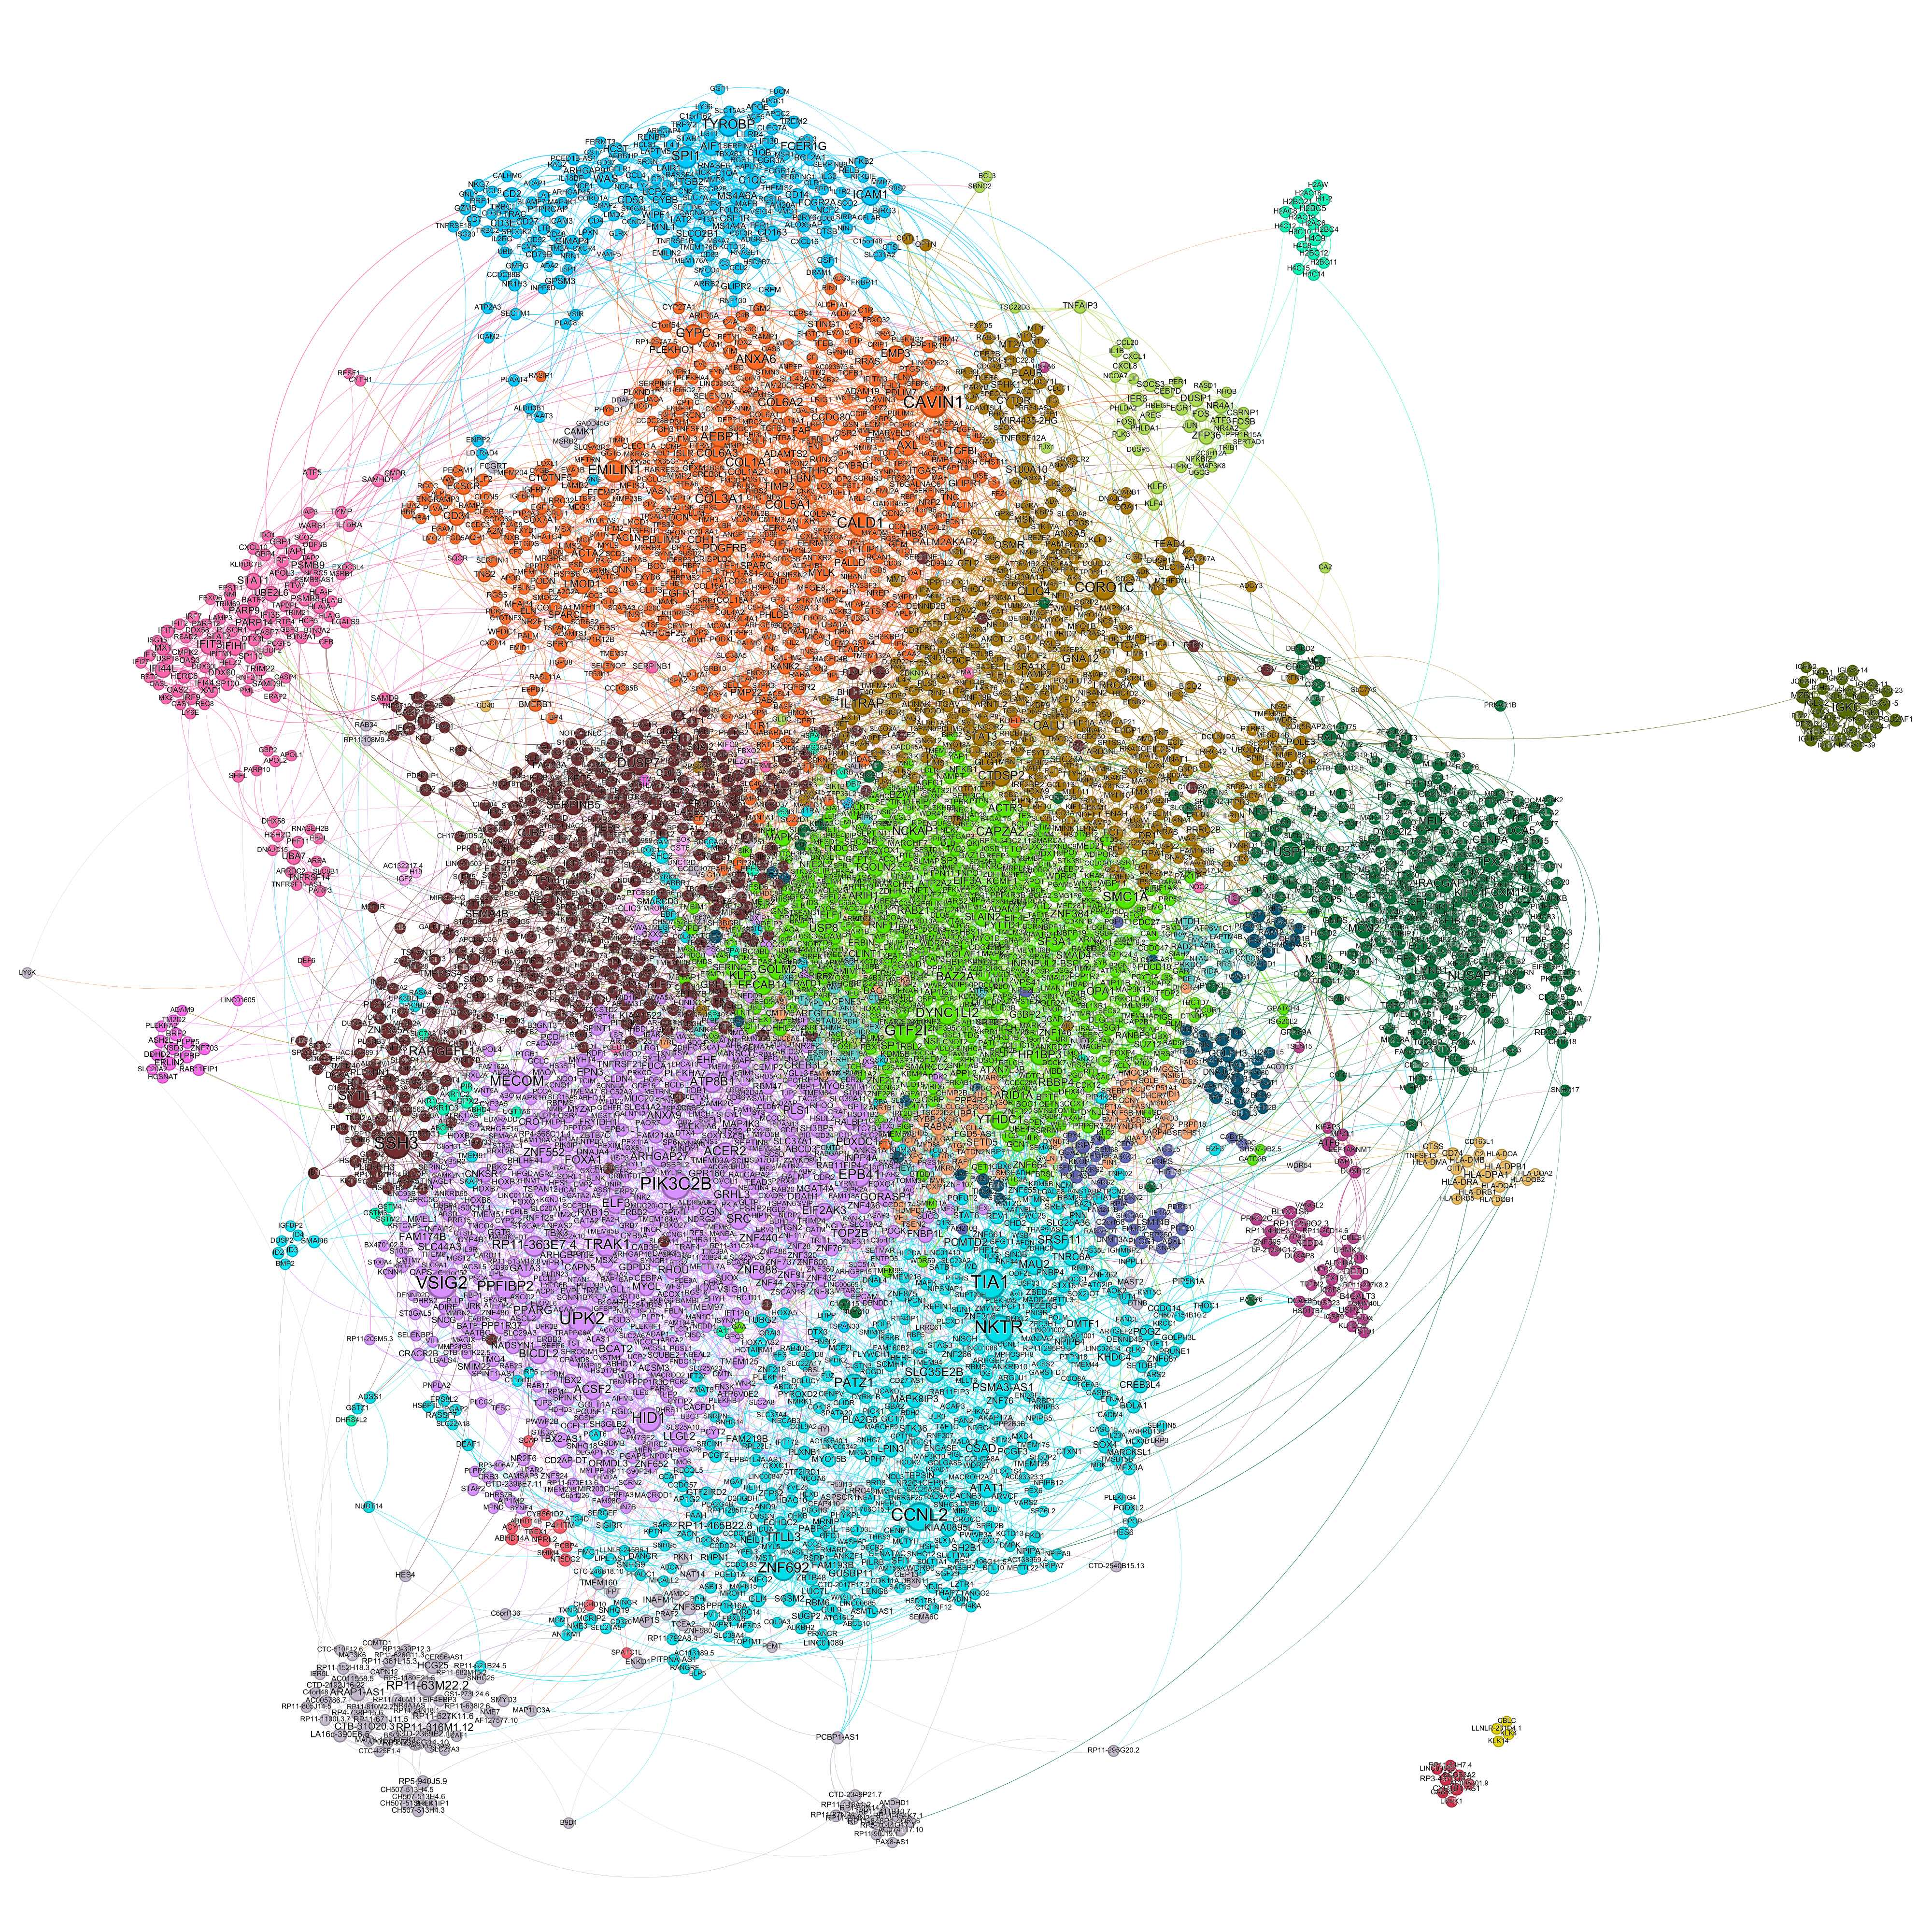
\includegraphics[width=0.9\paperwidth, height=0.9\paperheight, keepaspectratio]{Sections/Network_I/Resources/networks/tum_std_4K_6TF_lowRes.png} % Full-page image
  \parbox{0.8\textwidth}{\centering Network created from using the 5000 most varied genes in the tumour dataset, no weight modifier, minimum degree of 3 for standard genes and 6 for TF.}
\end{figure}
\restoregeometry
\newpage


\import{Sections/Network_I/}{tum.tex}

\newpage
\newgeometry{left=1.5cm, right=1.5cm, top=0.5cm, bottom=1cm}
\begin{figure}[p]
  \thispagestyle{empty} % Suppress the page number on this page
  \centering
  \captionsetup{justification=centering, labelfont=bf}
    \parbox{\textwidth}{\centering \Huge P0 derived Network - Leiden} 
    \vspace{3cm} % Space between title and image% 
        \label{fig:N_I:tum_P0}
    \includegraphics[width=0.9\paperwidth, height=0.9\paperheight, keepaspectratio]{Sections/Network_I/Resources/networks/p0_std_4K_50TF_2_lowRes.png} % Full-page image
    \parbox{0.8\textwidth}{\centering Network created from using the 4000 most varied genes in the P0 dataset, no weight modifier, minimum degree of 3 for standard genes and 50 for TF.}
\end{figure}
\restoregeometry
\newpage


\import{Sections/Network_I/}{p0.tex}


\section{Discussion}


This chapter presented a novel network approach developed to integrate both transcription factors and mutations into a co-expressed network which is then used for stratifying the \acrlong{mibc}. The research showed that modelling the edge weights proportional to gene mutation burden affect the network metrics, community detection methods and the MIBC subgroups. The selective edge pruning  acted as another data integration which influence the network metrics. Lastly, the P0 derived network showed potential to inform MIBC by finding different subgroups compared to the ones revealed by the tumour derived networks.

From the two set of networks the tumour derived seemed more responsive to the data integrated compared to the ones derived from the P0 samples. This might be explained by a limitation of the Leiden algorithm when a subset of genes is allowed a larger number of connections (50). Additionally, the P0 network is constructed from an incomplete representation of MIBC tumours, as it lacks a molecular representation of the basal (undifferentiated) group. Furthermore, when gap between the gene to sample representation is bridged only the expression in tumour is considered to stratify the MIBC without taking in account the abundance across the P0 samples. These limitations are addressed in \cref{s:N_II}, where the entire available non-tumour dataset is utilised, and a new version of MEV is introduced.


% Main takeaway 
Overall the experiment using both the tumour and P0 derived networks validates the initial hypothesis data integration can happen by modelling the number of edges and their weights. In addition, the non-tumour graphs showed that it is possible to form a non-tumour representation from which the MIBC can be derived. Next chapter explores in more depth the effects of selective edge pruning and differences between community detection algorithms into the tumour network

\subsection{Chapter contributions}

The research covered in this chapter was presented at the Complex Networks (CN) conference from Menton, France in 2023.

\begin{itemize}
    \item Validates the network approach as an integrative method for MIBC stratification
     \item Integration of the mutation burden and TF affect the network, community detection and MIBC stratification
     \item Network generated from the gene expression obtained from freshly isolated cells finds different groups from the tumour network representation
\end{itemize}
